%% slides_00_intro.tex — Title, outline, simple motivating example

\begin{frame}
\titlepage
\end{frame}

\begin{frame}{Outline}
\tableofcontents
\end{frame}

%%%%%%%%%%%%%%%%%%%%%%%%%%%%%%%%%%%%%%%%%%%%%%%%%%%%%%%%%%%%
\section{Motivation: A Simple Example}
%%%%%%%%%%%%%%%%%%%%%%%%%%%%%%%%%%%%%%%%%%%%%%%%%%%%%%%%%%%%

% ---------------------------------------------------------------------------
% ONE-SLIDE INTUITION: what is an MoE layer, in plain terms with concrete numbers
% ---------------------------------------------------------------------------
\begin{frame}{What Does an MoE Layer Actually Do? (Plain Example)}
\small
\textbf{Imagine you have 3 tokens and 4 specialists (experts). Each token picks 2 experts.}

\medskip
\begin{columns}[T]
\column{0.42\textwidth}

\begin{tikzpicture}[scale=0.82,transform shape,
  tok/.style={circle,draw=deepblue,fill=blue!12,minimum size=0.65cm,font=\tiny\bfseries},
  exp/.style={rectangle,draw=deepgreen,fill=green!10,rounded corners=3pt,
              minimum width=1.5cm,minimum height=0.55cm,font=\tiny\bfseries},
  arrow/.style={->,thick}]

  % tokens
  \node[tok] (t0) at (0, 0)    {$t_0$};
  \node[tok] (t1) at (0,-1.2)  {$t_1$};
  \node[tok] (t2) at (0,-2.4)  {$t_2$};

  % experts
  \node[exp] (e0) at (4, 0.3)  {Expert A};
  \node[exp] (e1) at (4,-0.8)  {Expert B};
  \node[exp] (e2) at (4,-1.9)  {Expert C};
  \node[exp] (e3) at (4,-3.0)  {Expert D};

  % routing arrows
  \draw[arrow,deepblue]   (t0) -- node[above,font=\tiny]{0.6} (e0);
  \draw[arrow,deepblue]   (t0) -- node[below,font=\tiny]{0.4} (e2);
  \draw[arrow,deepred]    (t1) -- node[above,font=\tiny]{0.7} (e1);
  \draw[arrow,deepred]    (t1) -- node[below,font=\tiny]{0.3} (e3);
  \draw[arrow,deepgreen]  (t2) -- node[above,font=\tiny]{0.5} (e0);
  \draw[arrow,deepgreen]  (t2) -- node[below,font=\tiny]{0.5} (e2);
\end{tikzpicture}

\column{0.55\textwidth}
\textbf{For each expert, gather its tokens, run a mini FFN, scatter back:}
\smallskip
\scriptsize
\begin{tabular}{c|l|l}
\toprule
Expert & Gets tokens & Contributes to \\
\midrule
A & $t_0\ (0.6),\ t_2\ (0.5)$ & $\text{out}[t_0], \text{out}[t_2]$ \\
B & $t_1\ (0.7)$ & $\text{out}[t_1]$ \\
C & $t_0\ (0.4),\ t_2\ (0.5)$ & $\text{out}[t_0], \text{out}[t_2]$ \\
D & $t_1\ (0.3)$ & $\text{out}[t_1]$ \\
\bottomrule
\end{tabular}

\medskip
\[
\text{out}[t_0] = 0.6 \cdot \text{FFN}_A(t_0) + 0.4 \cdot \text{FFN}_C(t_0)
\]
\[
\text{out}[t_1] = 0.7 \cdot \text{FFN}_B(t_1) + 0.3 \cdot \text{FFN}_D(t_1)
\]

\vspace{4pt}
\begin{alertblock}{\scriptsize The challenge at scale}
\scriptsize
In DeepSeek: $T$ up to 14\,000, 256 experts, top-8 selection.\\
Each FFN: $7168\times4096$ FP8 matrix. Sequential = \textbf{too slow}.
\end{alertblock}
\end{columns}
\end{frame}

% ---------------------------------------------------------------------------
\begin{frame}{The FFN Inside Each Expert}
\small
\textbf{Each expert runs the same structure — a gated feed-forward network:}

\medskip
\begin{columns}[T]
\column{0.52\textwidth}

\begin{enumerate}\small
  \item \textbf{GEMM1} — Project to gate+up space:
    \[ A_e \cdot W_1^\top \;\to\; [T_k,\; 4096] \]
    $W_1$ stores \emph{both} gate and up rows concatenated.

  \item \textbf{SwiGLU} — Gated activation:
    \[ C = \underbrace{Y[:, 0{:}2048]}_{\text{gate}} \odot \text{silu}\!\left(\underbrace{Y[:,2048{:}]}_{\text{up}}\right) \]
    Output: $[T_k, 2048]$. Smooth on/off switch per dimension.

  \item \textbf{GEMM2} — Project back to hidden:
    \[ C \cdot W_2^\top \;\to\; [T_k,\; 7168] \]
\end{enumerate}

\column{0.45\textwidth}
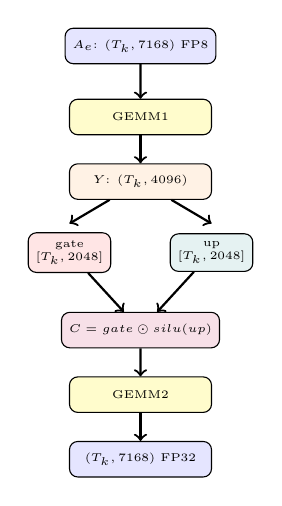
\begin{tikzpicture}[scale=0.82,transform shape,
  box/.style={rectangle,draw,rounded corners=3pt,font=\tiny,
              align=center,minimum height=0.55cm,minimum width=2.2cm},
  arrow/.style={->,thick}]
\node[box,fill=blue!10]   (a)    at(0,0)    {$A_e$: $(T_k,7168)$ FP8};
\node[box,fill=yellow!20] (g1)   at(0,-1.1) {GEMM1};
\node[box,fill=orange!10] (y)    at(0,-2.1) {$Y$: $(T_k,4096)$};
\node[box,fill=red!10,minimum width=0.95cm]
                          (gate) at(-1.1,-3.2){gate\\$[T_k,2048]$};
\node[box,fill=teal!10,minimum width=0.95cm]
                          (up)   at(1.1,-3.2) {up\\$[T_k,2048]$};
\node[box,fill=purple!12] (act)  at(0,-4.4) {$C=\text{gate}\odot\text{silu(up)}$};
\node[box,fill=yellow!20] (g2)   at(0,-5.4) {GEMM2};
\node[box,fill=blue!10]   (o)    at(0,-6.4) {$(T_k,7168)$ FP32};
\draw[arrow](a)--(g1); \draw[arrow](g1)--(y);
\draw[arrow](y)--(-1.1,-2.75); \draw[arrow](y)--(1.1,-2.75);
\draw[arrow](gate)--(act); \draw[arrow](up)--(act);
\draw[arrow](act)--(g2); \draw[arrow](g2)--(o);
\end{tikzpicture}
\end{columns}
\end{frame}
